%proportional corrected algorithm methods
\subsubsection*{Algorithm}
We attempted to correct the dark spot issue by significantly reducing the absolute difference between dark pixels and the average colour, ensuring that the dark spots would instead have colours close to the average. We perform this correction on the output of the proportional adjustment algorithm.

\begin{equation} \label{eq:prop_corr_algo}
  r'' = \left.
  \begin{dcases}
    \displaystyle \mean{r'} - \frac{(\mean{r'} - r')}{\alpha}, & \text{for } r' < \mean{r'} \\
    \displaystyle r', & \text{for } r' \geq \mean{r'} \\
  \end{dcases}
  \right.\\
\end{equation}

\nomenclature{$r''$}{Value of the red channel of the pixel after a second algorithm is applied.}
\nomenclature{$\mean{r'}$}{Average value of the red channel of the hand image outputted by the first algorithm.}

Where $\alpha$ is a constant, $\alpha  > 1$. The same equation applies for the $g$ and $b$ channels.

\subsubsection*{Results}

In Table \ref{tab:prop_correct_test_a1p1} we show the results for colour transfers between all possible combinations of our test images.
\begin{longtable}{|N||c|c|c|}
	\caption{Test results of proportional brightening with correction for dark spots, alpha = 1.1\label{tab:prop_correct_test_a1p1}}\\
	\hline
	\multicolumn{1}{|c||}{No.} & Original & Target & Results \\ 
	\hline
	    \label{row:prop_correct_test_a1p1_hand_dark_to_hand_brown} &
  \begin{minipage}{.29\textwidth}
    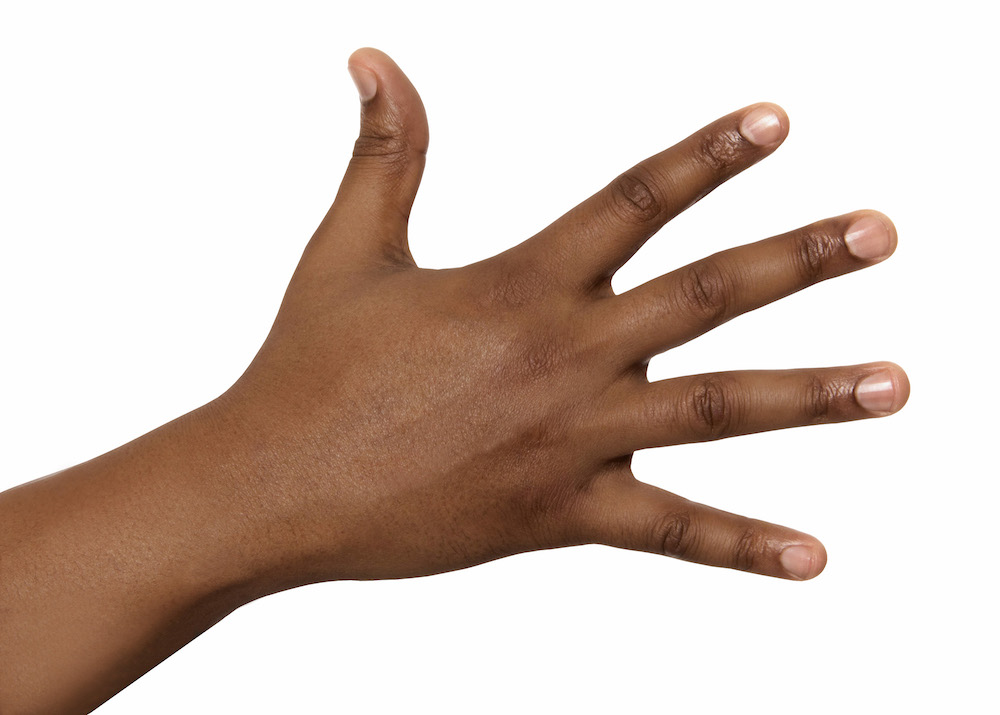
\includegraphics[width=\textwidth,height=\textheight,keepaspectratio]{../inputs/hand_dark.jpg}
  \end{minipage} & 
  \begin{minipage}{.29\textwidth}
    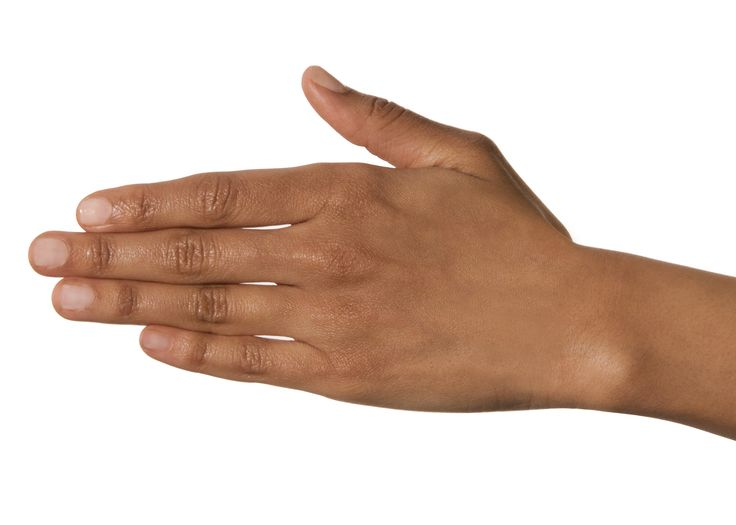
\includegraphics[width=\textwidth,height=\textheight,keepaspectratio]{../inputs/hand_brown.jpg}
  \end{minipage} & 
  \begin{minipage}{.29\textwidth}
    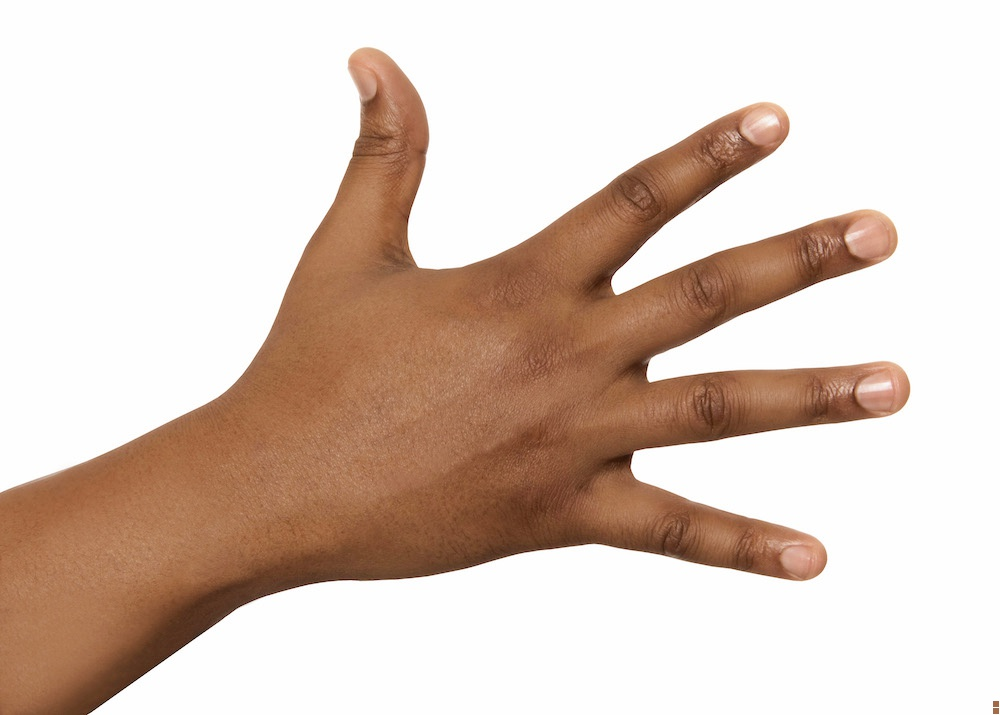
\includegraphics[width=\textwidth,height=\textheight,keepaspectratio]{../rc_test/outputs/20170522_proportional_corrected_test_alpha1p1/hand_dark_to_hand_brown.jpg}
  \end{minipage} \\
\hline  \label{row:prop_correct_test_a1p1_hand_dark_to_hand_light} &
  \begin{minipage}{.29\textwidth}
    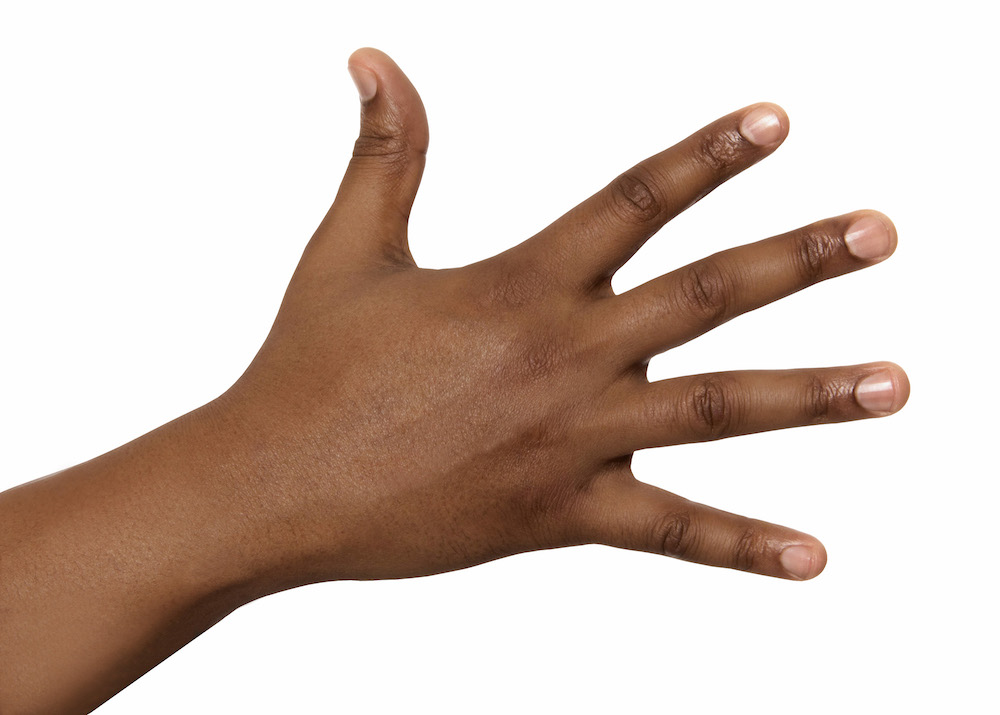
\includegraphics[width=\textwidth,height=\textheight,keepaspectratio]{../inputs/hand_dark.jpg}
  \end{minipage} & 
  \begin{minipage}{.29\textwidth}
    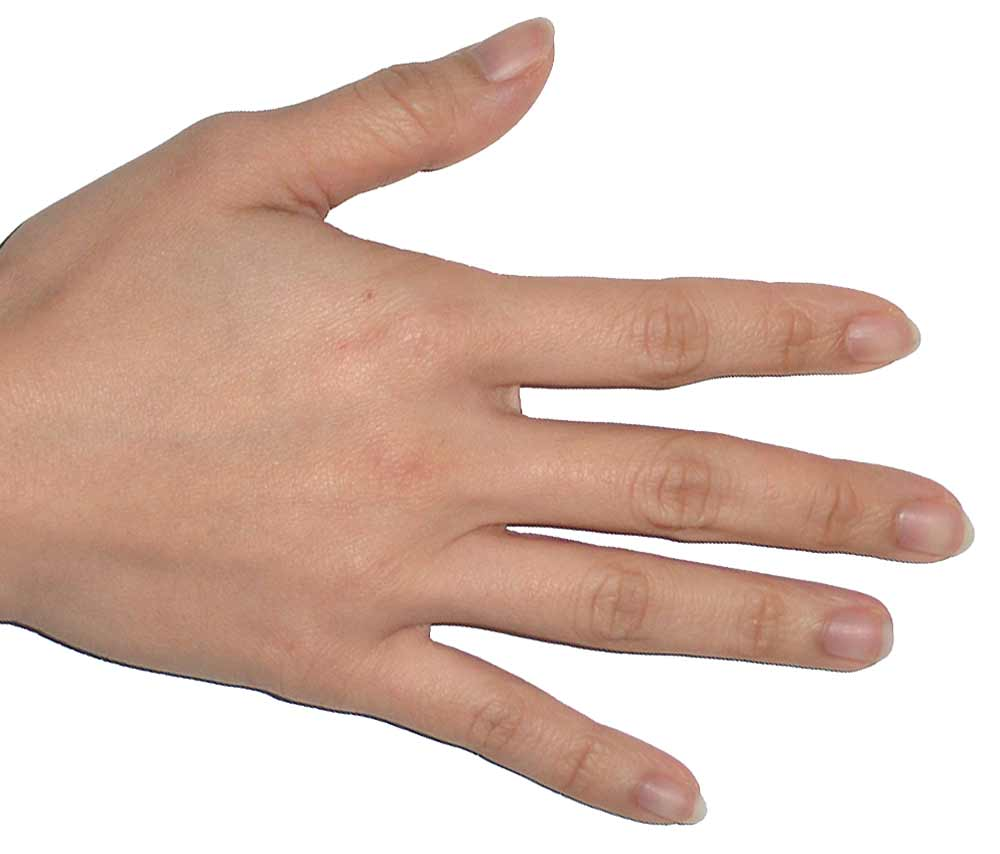
\includegraphics[width=\textwidth,height=\textheight,keepaspectratio]{../inputs/hand_light.jpg}
  \end{minipage} & 
  \begin{minipage}{.29\textwidth}
    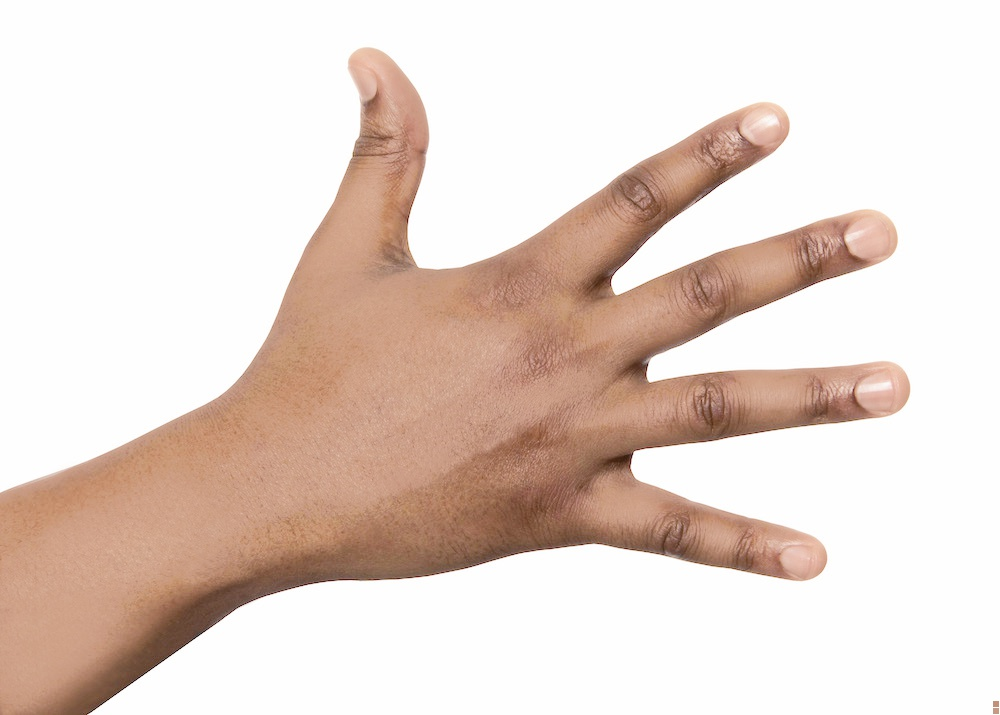
\includegraphics[width=\textwidth,height=\textheight,keepaspectratio]{../rc_test/outputs/20170522_proportional_corrected_test_alpha1p1/hand_dark_to_hand_light.jpg}
  \end{minipage} \\
\hline  \label{row:prop_correct_test_a1p1_hand_dark_to_hand_pale} &
  \begin{minipage}{.29\textwidth}
    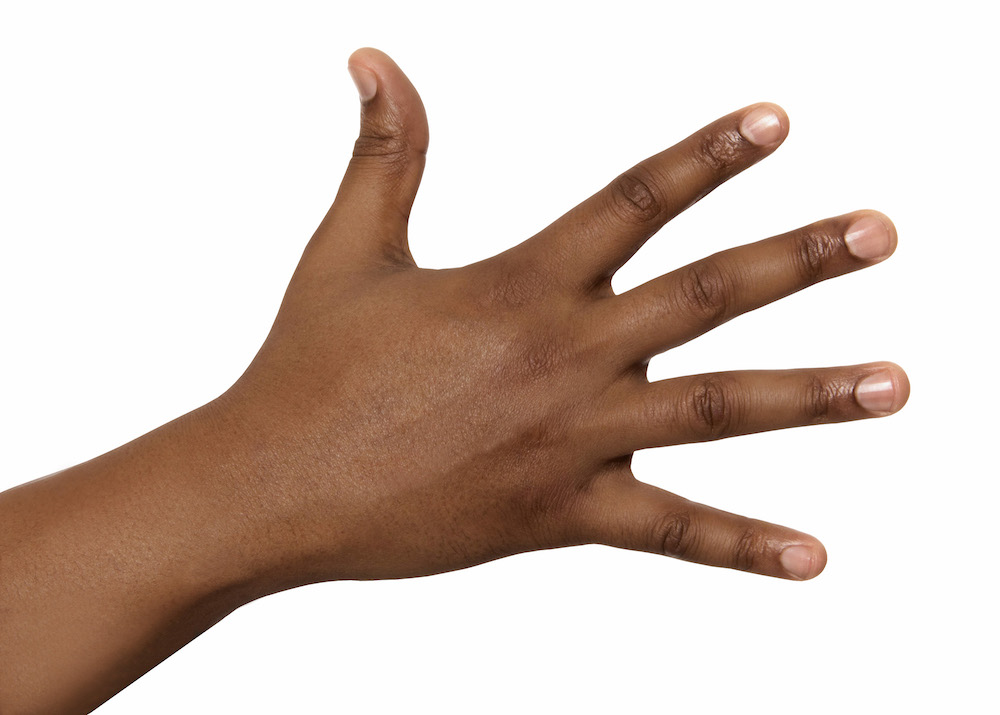
\includegraphics[width=\textwidth,height=\textheight,keepaspectratio]{../inputs/hand_dark.jpg}
  \end{minipage} & 
  \begin{minipage}{.29\textwidth}
    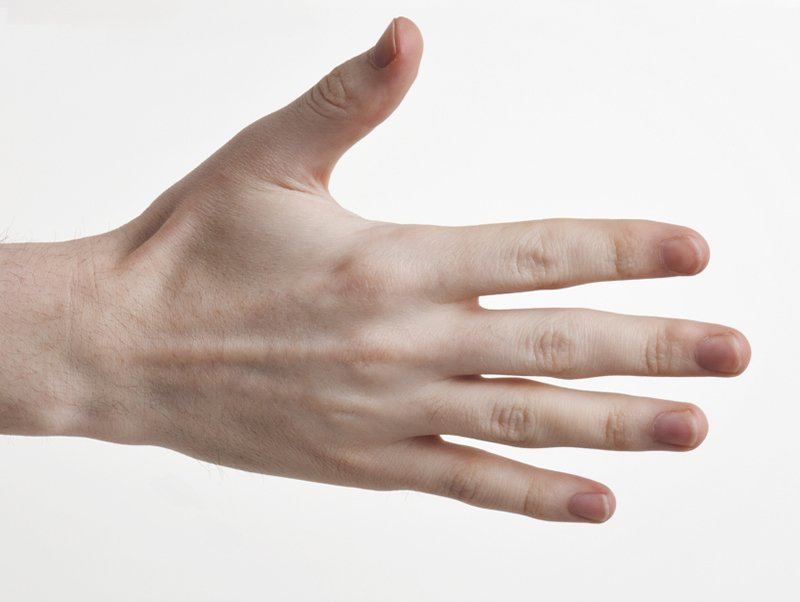
\includegraphics[width=\textwidth,height=\textheight,keepaspectratio]{../inputs/hand_pale.jpg}
  \end{minipage} & 
  \begin{minipage}{.29\textwidth}
    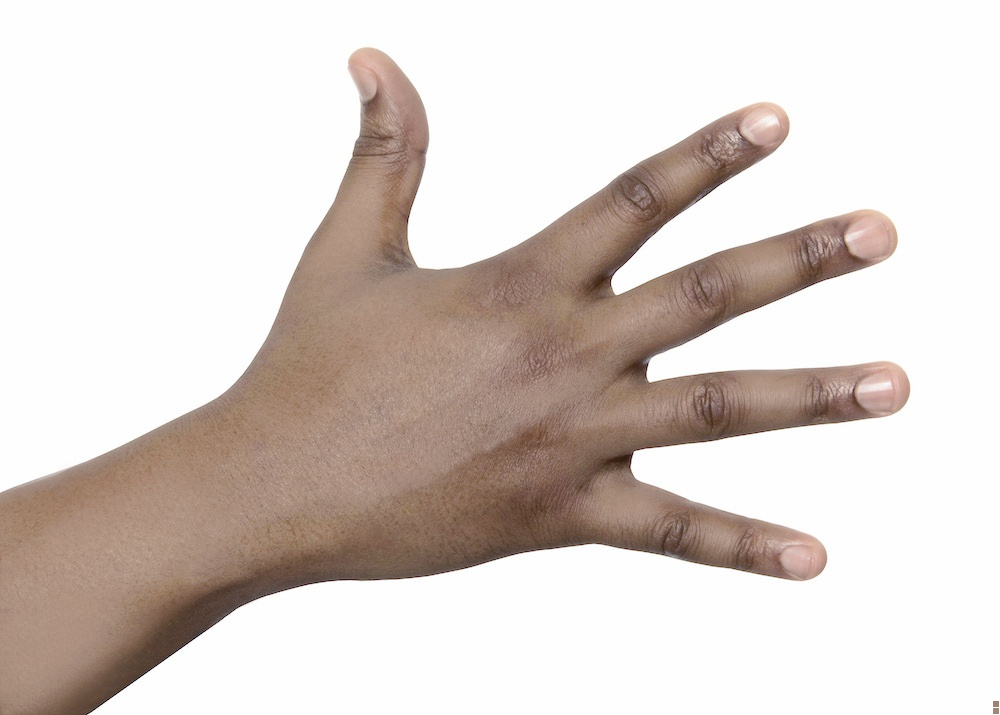
\includegraphics[width=\textwidth,height=\textheight,keepaspectratio]{../rc_test/outputs/20170522_proportional_corrected_test_alpha1p1/hand_dark_to_hand_pale.jpg}
  \end{minipage} \\
\hline  \label{row:prop_correct_test_a1p1_hand_brown_to_hand_dark} &
  \begin{minipage}{.29\textwidth}
    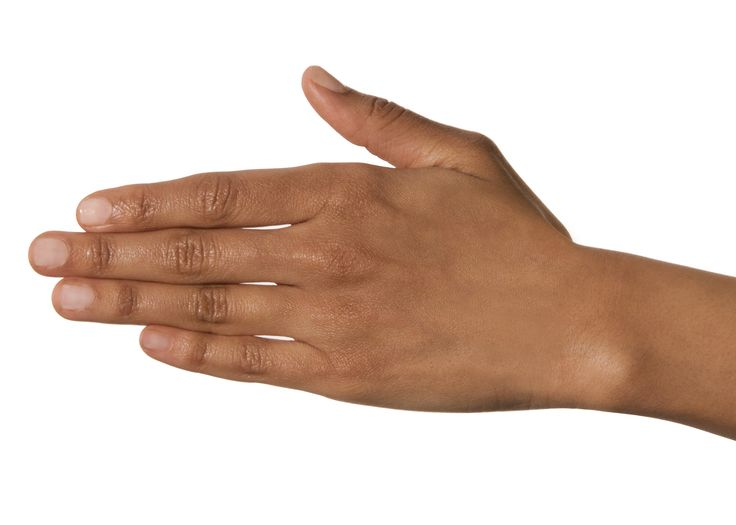
\includegraphics[width=\textwidth,height=\textheight,keepaspectratio]{../inputs/hand_brown.jpg}
  \end{minipage} & 
  \begin{minipage}{.29\textwidth}
    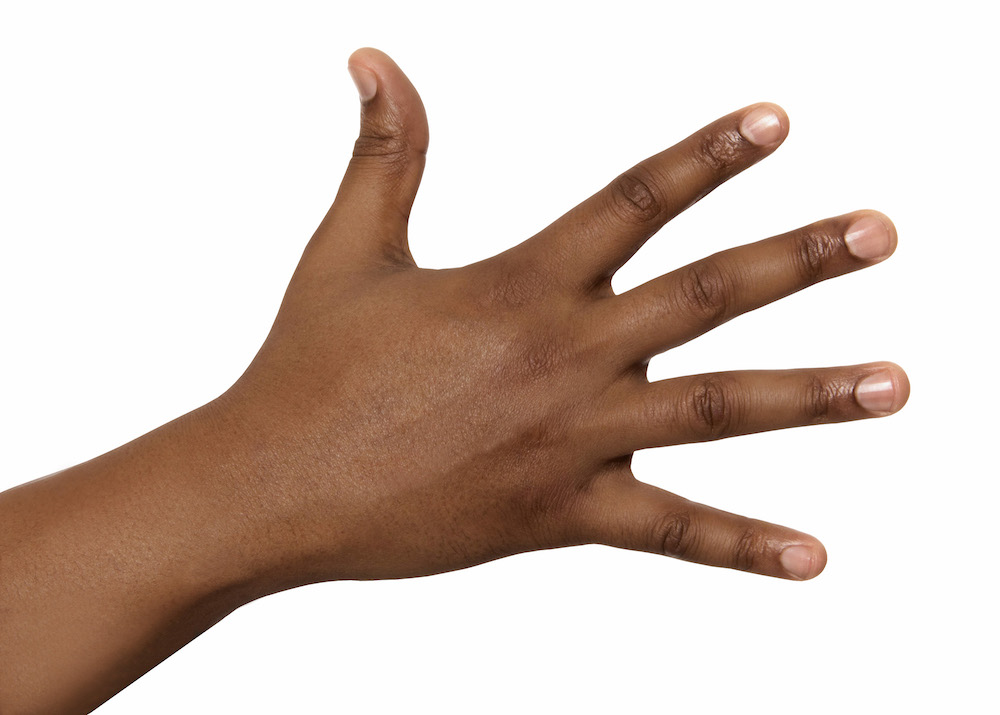
\includegraphics[width=\textwidth,height=\textheight,keepaspectratio]{../inputs/hand_dark.jpg}
  \end{minipage} & 
  \begin{minipage}{.29\textwidth}
    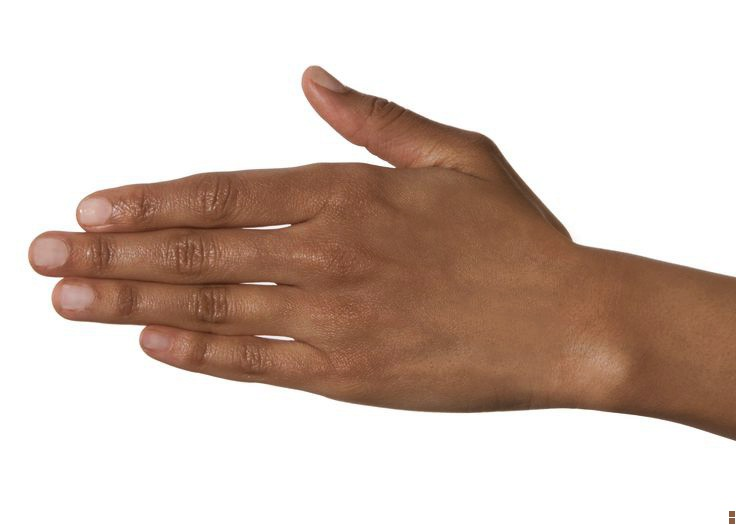
\includegraphics[width=\textwidth,height=\textheight,keepaspectratio]{../rc_test/outputs/20170522_proportional_corrected_test_alpha1p1/hand_brown_to_hand_dark.jpg}
  \end{minipage} \\
\hline  \label{row:prop_correct_test_a1p1_hand_brown_to_hand_light} &
  \begin{minipage}{.29\textwidth}
    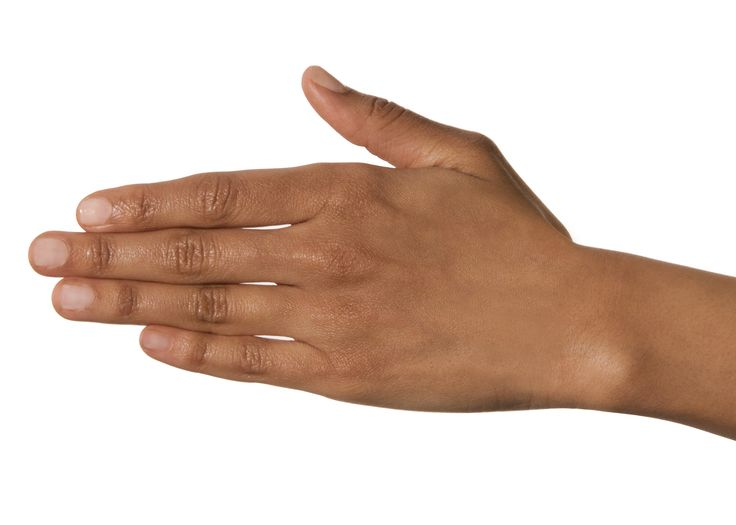
\includegraphics[width=\textwidth,height=\textheight,keepaspectratio]{../inputs/hand_brown.jpg}
  \end{minipage} & 
  \begin{minipage}{.29\textwidth}
    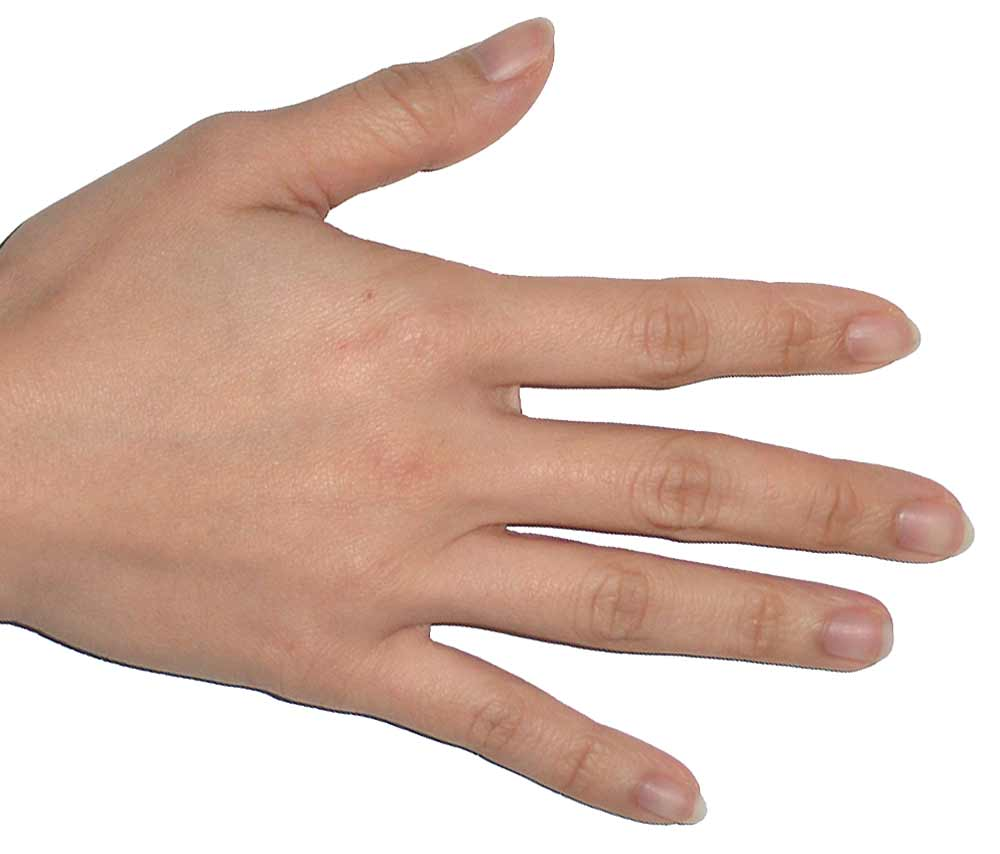
\includegraphics[width=\textwidth,height=\textheight,keepaspectratio]{../inputs/hand_light.jpg}
  \end{minipage} & 
  \begin{minipage}{.29\textwidth}
    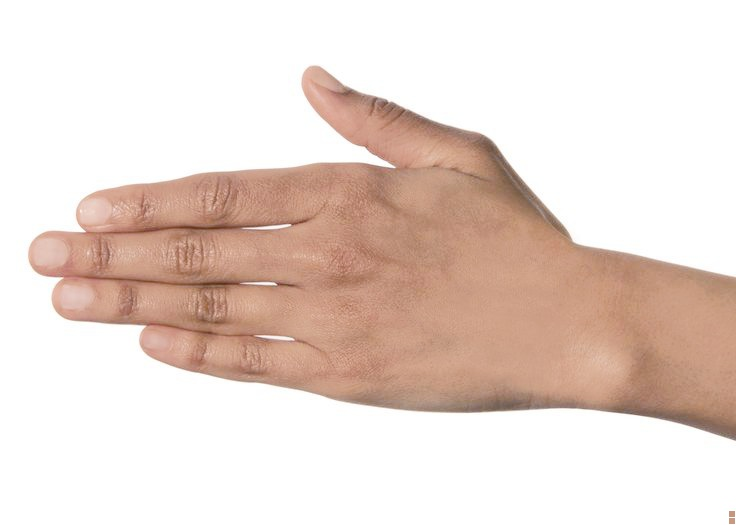
\includegraphics[width=\textwidth,height=\textheight,keepaspectratio]{../rc_test/outputs/20170522_proportional_corrected_test_alpha1p1/hand_brown_to_hand_light.jpg}
  \end{minipage} \\
\hline  \label{row:prop_correct_test_a1p1_hand_brown_to_hand_pale} &
  \begin{minipage}{.29\textwidth}
    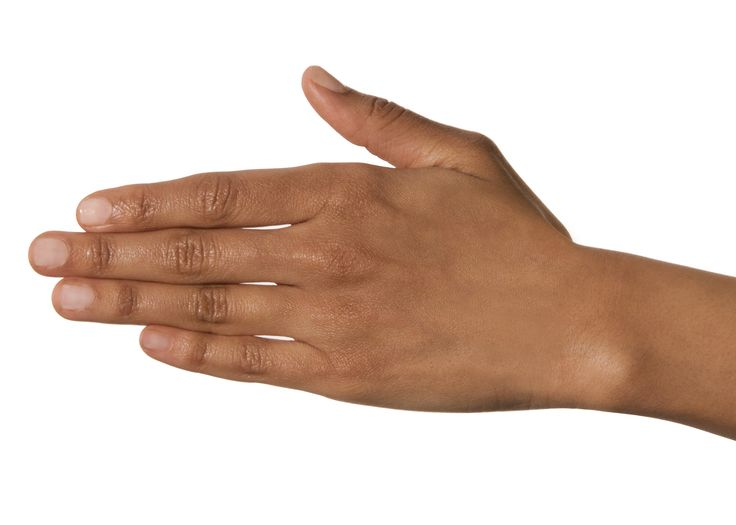
\includegraphics[width=\textwidth,height=\textheight,keepaspectratio]{../inputs/hand_brown.jpg}
  \end{minipage} & 
  \begin{minipage}{.29\textwidth}
    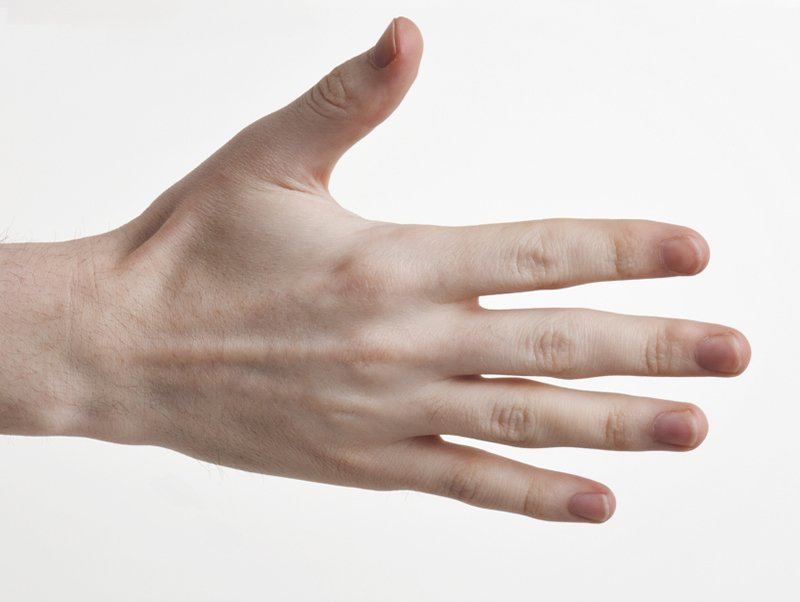
\includegraphics[width=\textwidth,height=\textheight,keepaspectratio]{../inputs/hand_pale.jpg}
  \end{minipage} & 
  \begin{minipage}{.29\textwidth}
    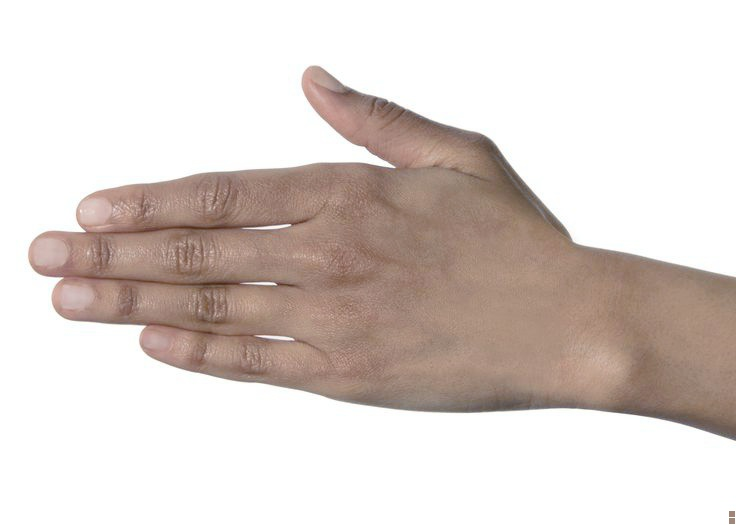
\includegraphics[width=\textwidth,height=\textheight,keepaspectratio]{../rc_test/outputs/20170522_proportional_corrected_test_alpha1p1/hand_brown_to_hand_pale.jpg}
  \end{minipage} \\
\hline  \label{row:prop_correct_test_a1p1_hand_light_to_hand_dark} &
  \begin{minipage}{.29\textwidth}
    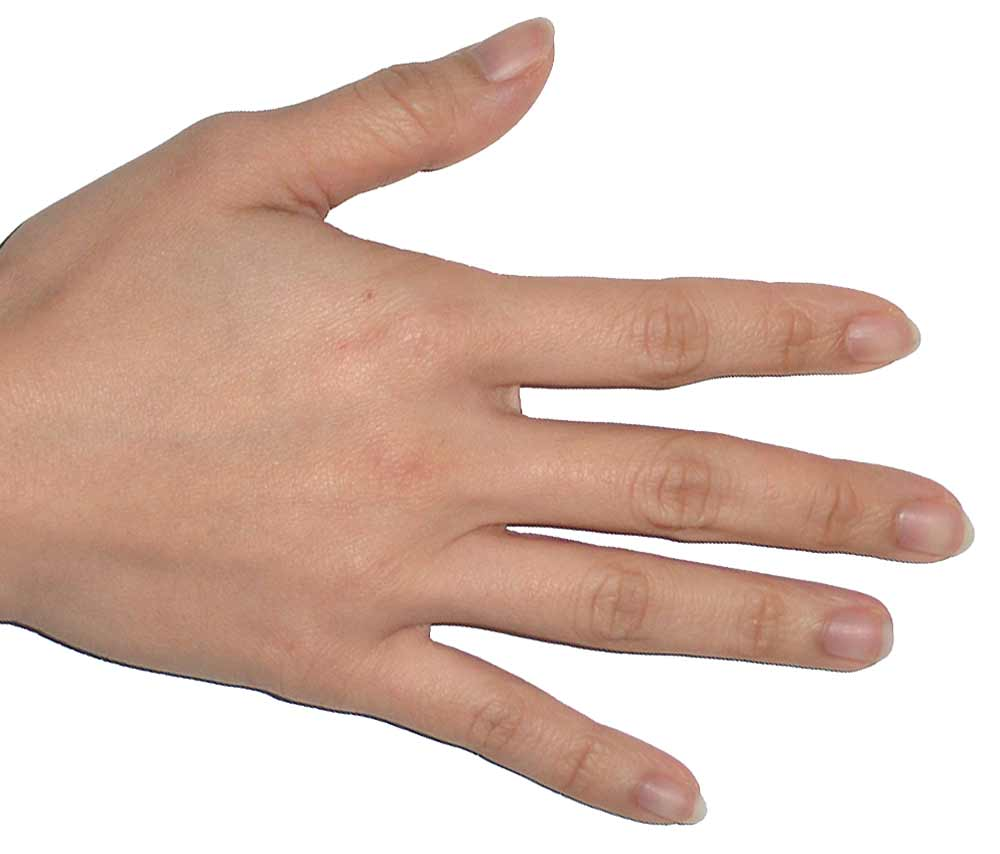
\includegraphics[width=\textwidth,height=\textheight,keepaspectratio]{../inputs/hand_light.jpg}
  \end{minipage} & 
  \begin{minipage}{.29\textwidth}
    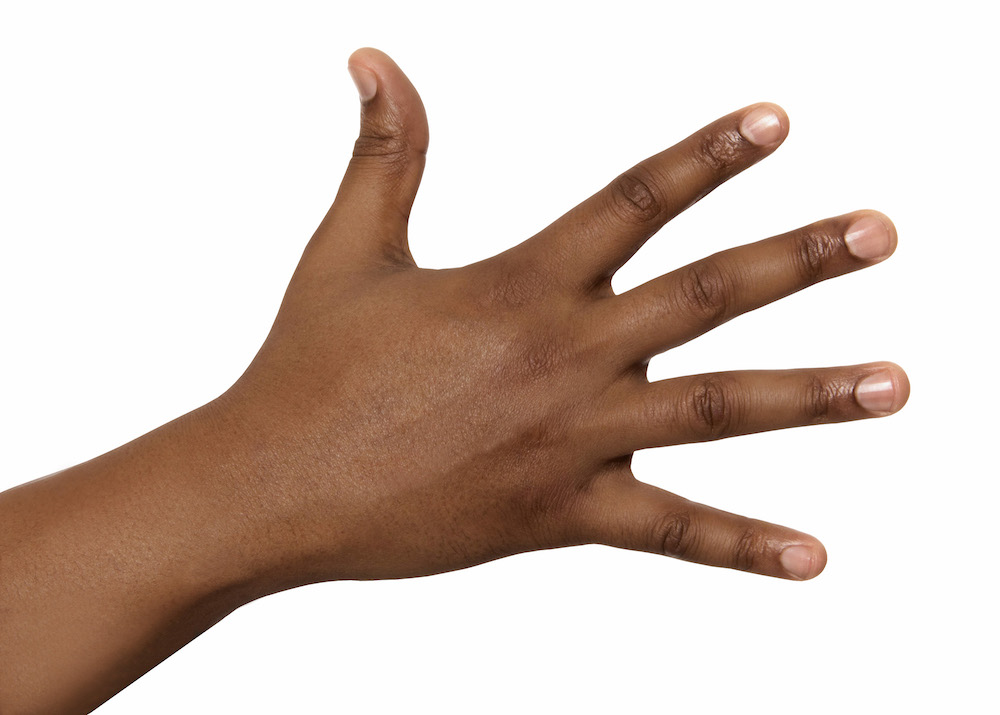
\includegraphics[width=\textwidth,height=\textheight,keepaspectratio]{../inputs/hand_dark.jpg}
  \end{minipage} & 
  \begin{minipage}{.29\textwidth}
    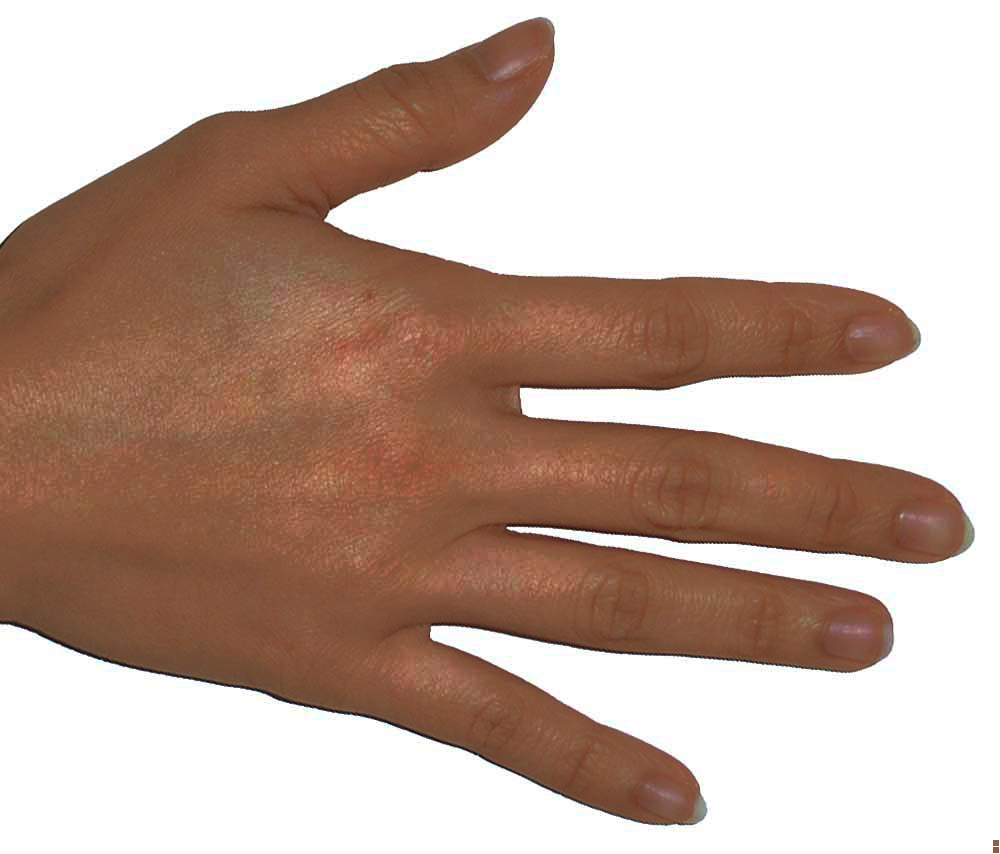
\includegraphics[width=\textwidth,height=\textheight,keepaspectratio]{../rc_test/outputs/20170522_proportional_corrected_test_alpha1p1/hand_light_to_hand_dark.jpg}
  \end{minipage} \\
\hline  \label{row:prop_correct_test_a1p1_hand_light_to_hand_brown} &
  \begin{minipage}{.29\textwidth}
    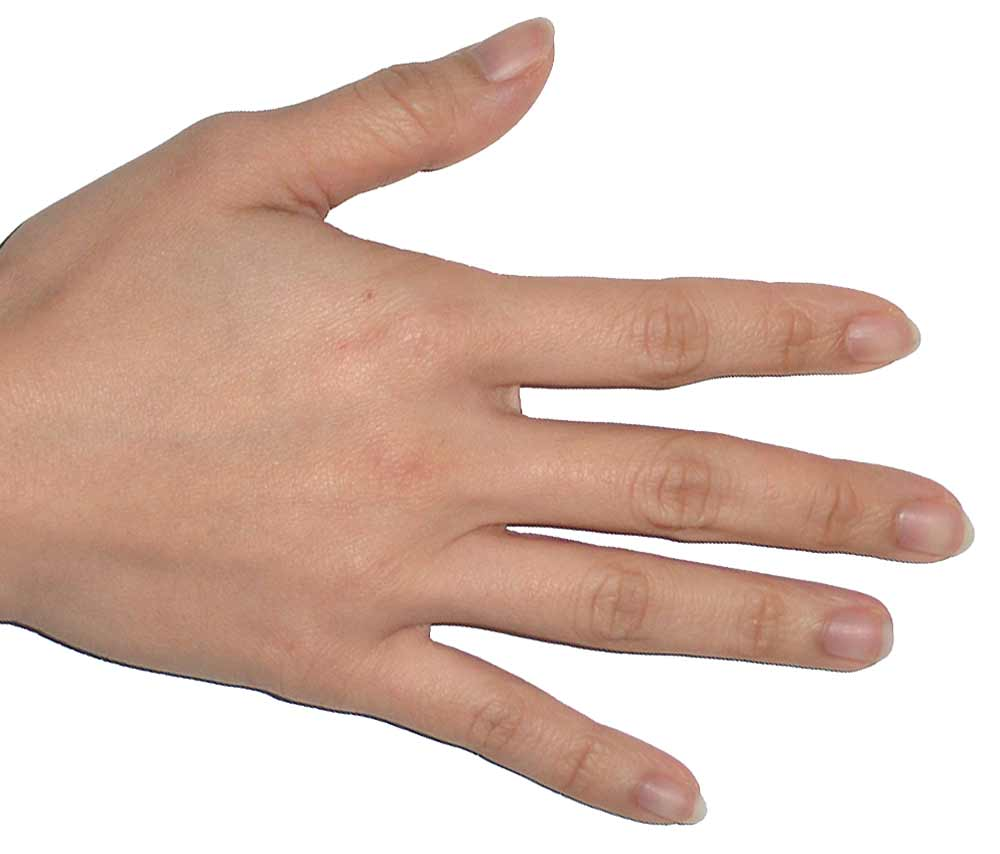
\includegraphics[width=\textwidth,height=\textheight,keepaspectratio]{../inputs/hand_light.jpg}
  \end{minipage} & 
  \begin{minipage}{.29\textwidth}
    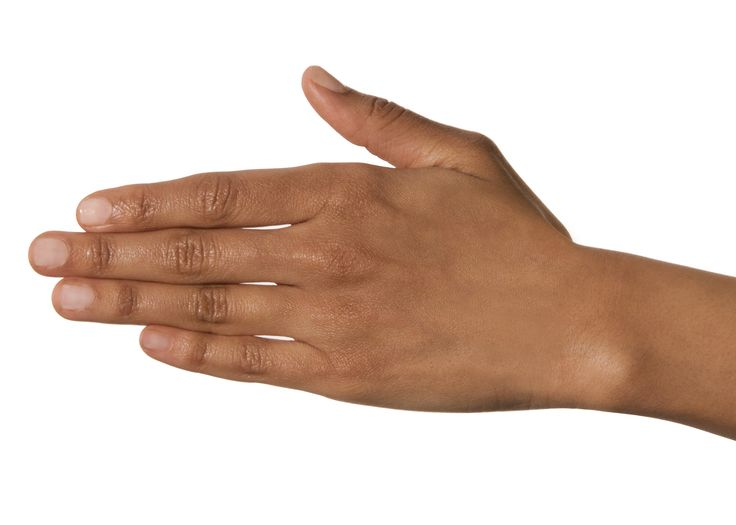
\includegraphics[width=\textwidth,height=\textheight,keepaspectratio]{../inputs/hand_brown.jpg}
  \end{minipage} & 
  \begin{minipage}{.29\textwidth}
    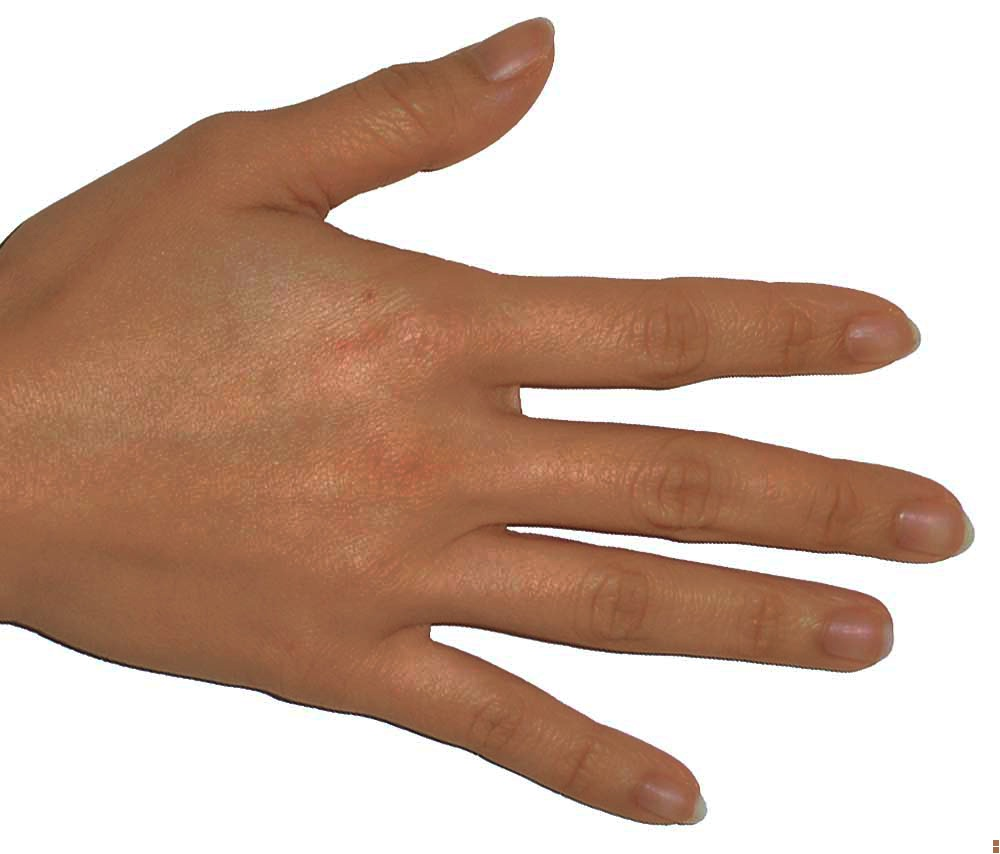
\includegraphics[width=\textwidth,height=\textheight,keepaspectratio]{../rc_test/outputs/20170522_proportional_corrected_test_alpha1p1/hand_light_to_hand_brown.jpg}
  \end{minipage} \\
\hline  \label{row:prop_correct_test_a1p1_hand_light_to_hand_pale} &
  \begin{minipage}{.29\textwidth}
    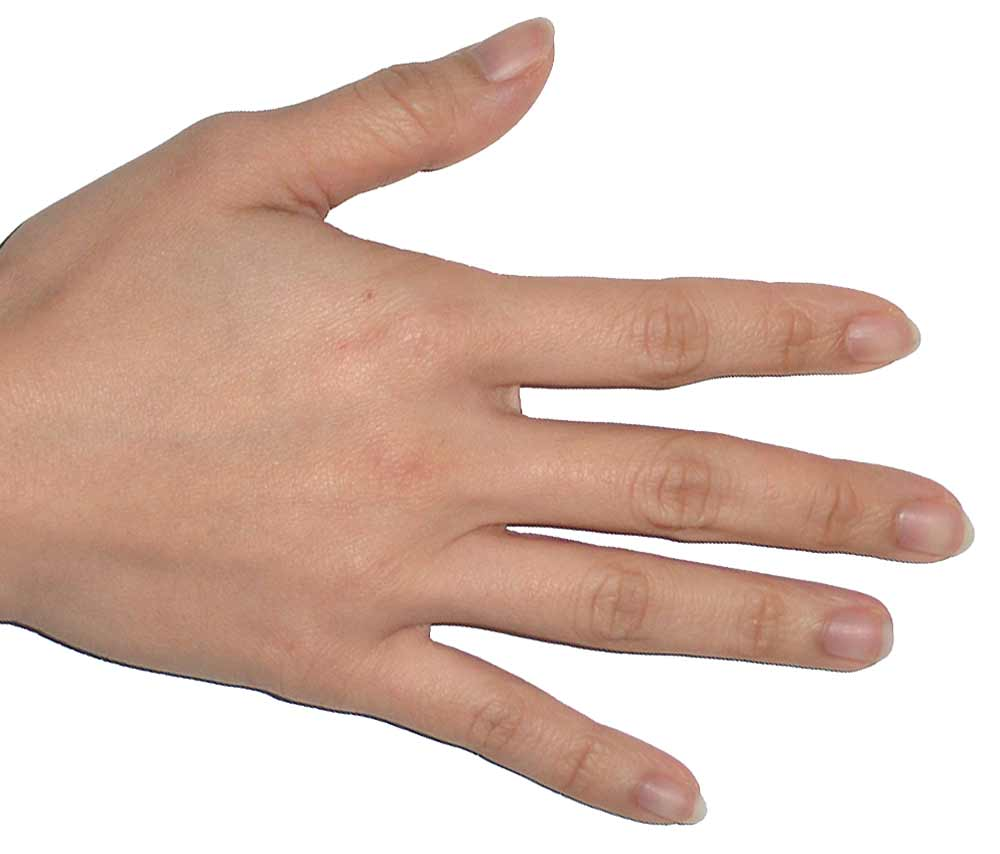
\includegraphics[width=\textwidth,height=\textheight,keepaspectratio]{../inputs/hand_light.jpg}
  \end{minipage} & 
  \begin{minipage}{.29\textwidth}
    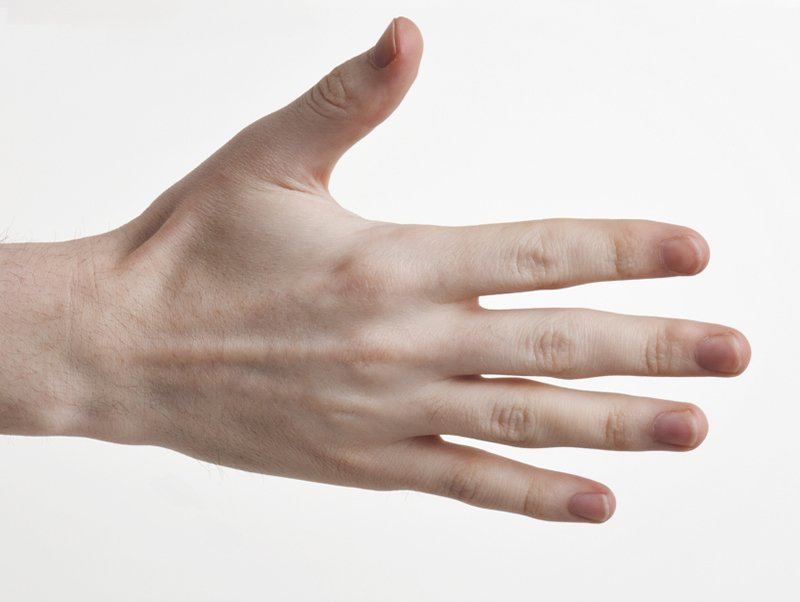
\includegraphics[width=\textwidth,height=\textheight,keepaspectratio]{../inputs/hand_pale.jpg}
  \end{minipage} & 
  \begin{minipage}{.29\textwidth}
    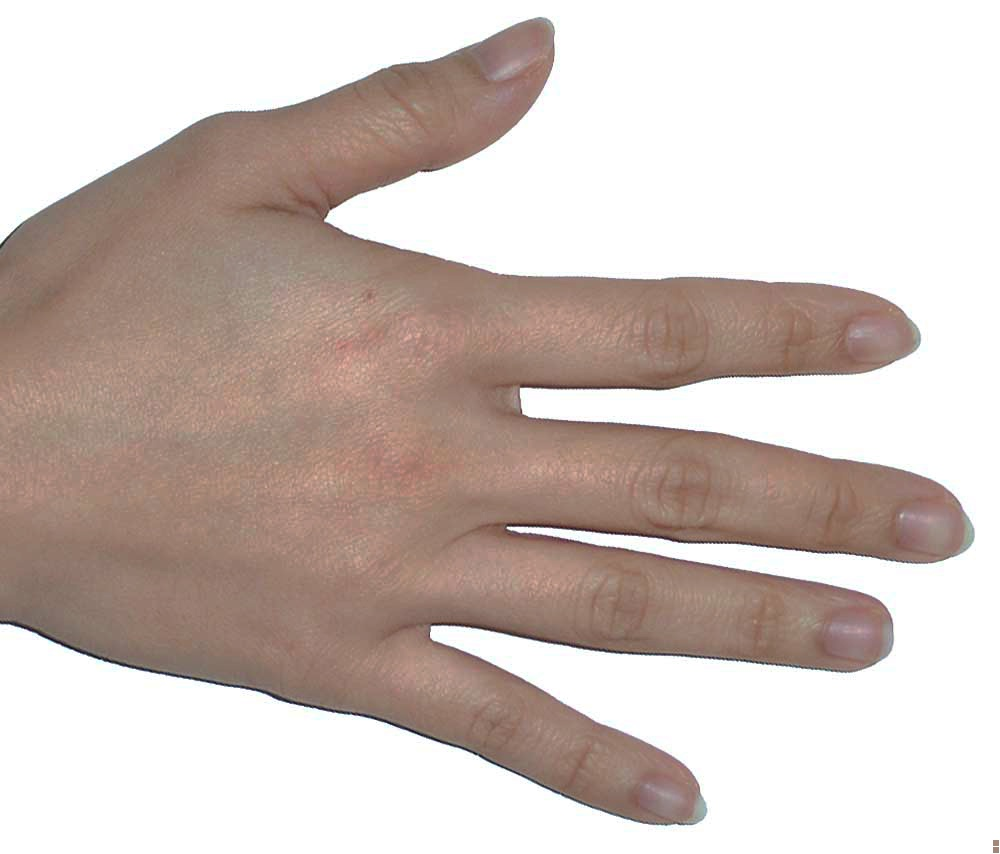
\includegraphics[width=\textwidth,height=\textheight,keepaspectratio]{../rc_test/outputs/20170522_proportional_corrected_test_alpha1p1/hand_light_to_hand_pale.jpg}
  \end{minipage} \\
\hline  \label{row:prop_correct_test_a1p1_hand_pale_to_hand_dark} &
  \begin{minipage}{.29\textwidth}
    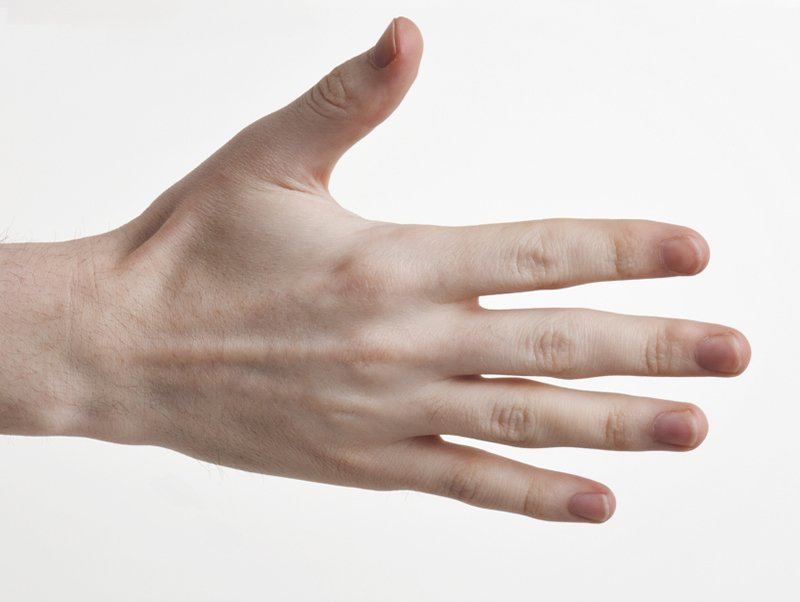
\includegraphics[width=\textwidth,height=\textheight,keepaspectratio]{../inputs/hand_pale.jpg}
  \end{minipage} & 
  \begin{minipage}{.29\textwidth}
    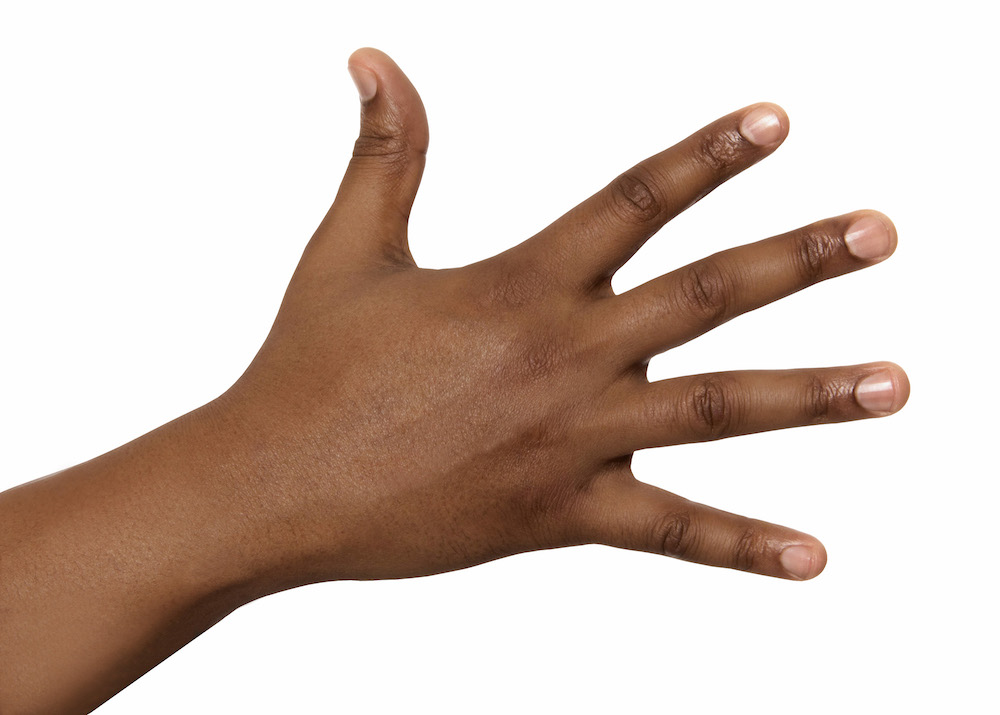
\includegraphics[width=\textwidth,height=\textheight,keepaspectratio]{../inputs/hand_dark.jpg}
  \end{minipage} & 
  \begin{minipage}{.29\textwidth}
    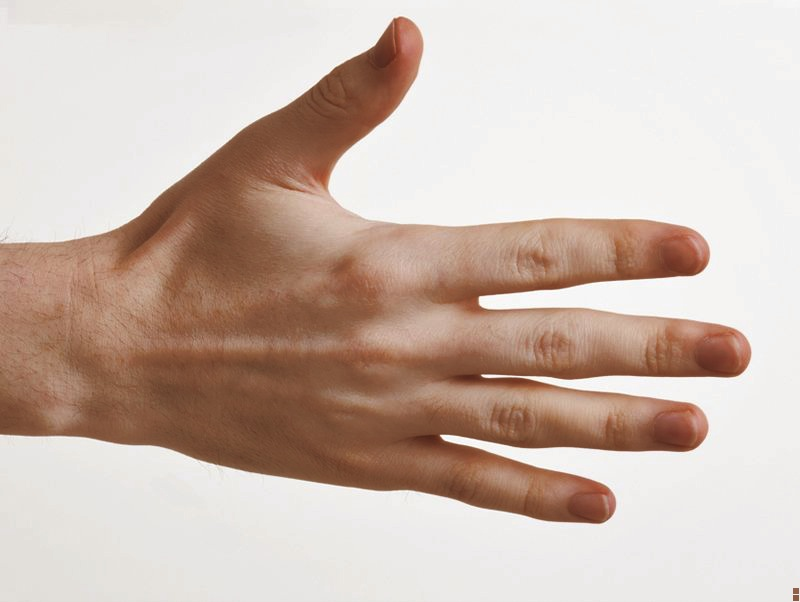
\includegraphics[width=\textwidth,height=\textheight,keepaspectratio]{../rc_test/outputs/20170522_proportional_corrected_test_alpha1p1/hand_pale_to_hand_dark.jpg}
  \end{minipage} \\
\hline  \label{row:prop_correct_test_a1p1_hand_pale_to_hand_brown} &
  \begin{minipage}{.29\textwidth}
    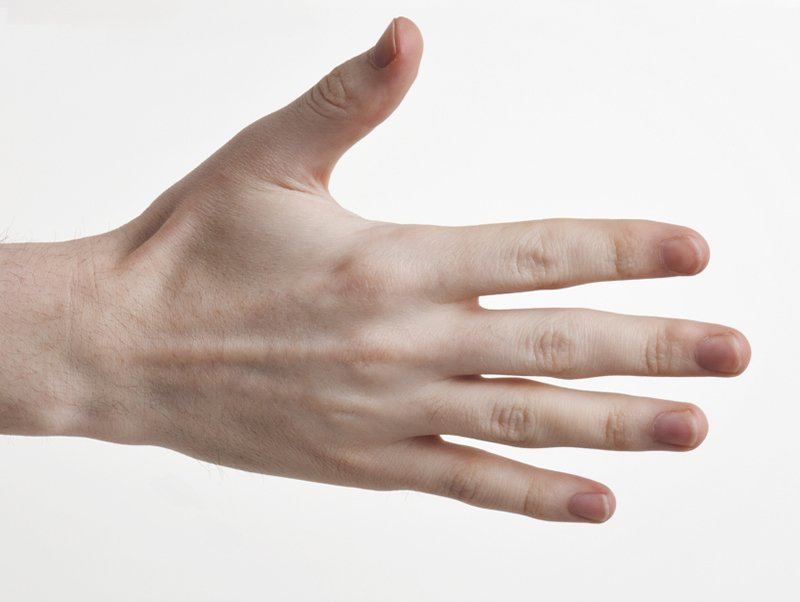
\includegraphics[width=\textwidth,height=\textheight,keepaspectratio]{../inputs/hand_pale.jpg}
  \end{minipage} & 
  \begin{minipage}{.29\textwidth}
    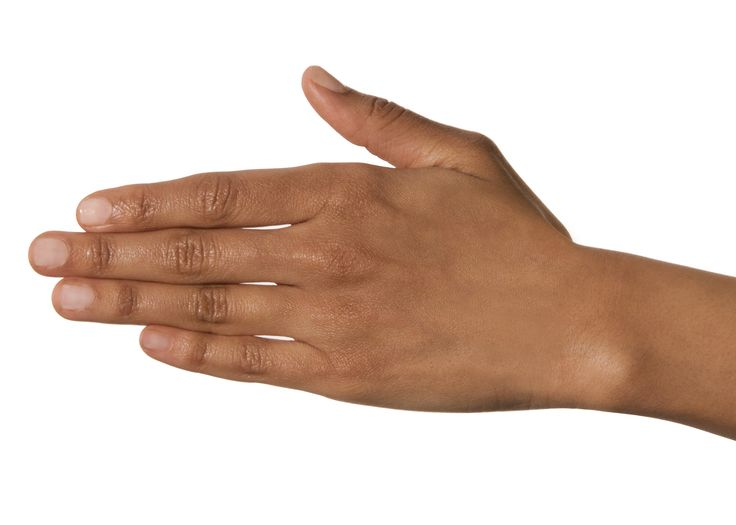
\includegraphics[width=\textwidth,height=\textheight,keepaspectratio]{../inputs/hand_brown.jpg}
  \end{minipage} & 
  \begin{minipage}{.29\textwidth}
    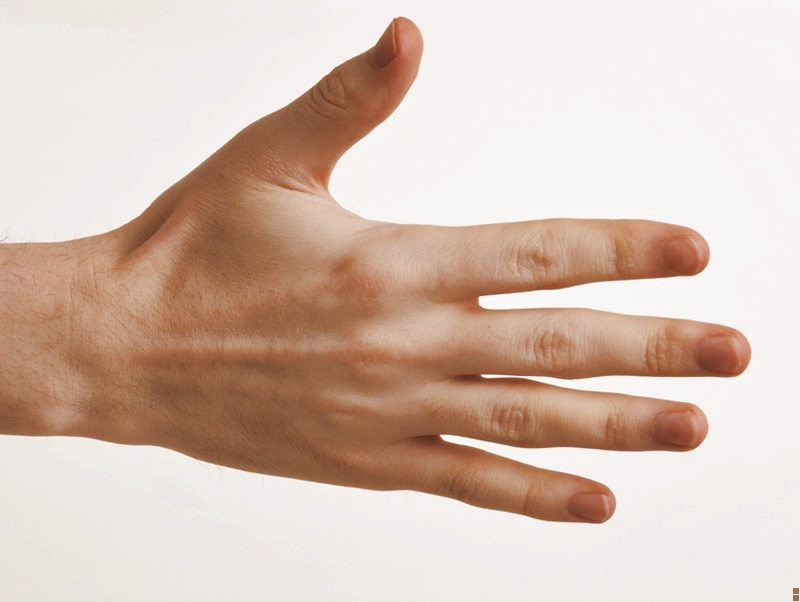
\includegraphics[width=\textwidth,height=\textheight,keepaspectratio]{../rc_test/outputs/20170522_proportional_corrected_test_alpha1p1/hand_pale_to_hand_brown.jpg}
  \end{minipage} \\
\hline  \label{row:prop_correct_test_a1p1_hand_pale_to_hand_light} &
  \begin{minipage}{.29\textwidth}
    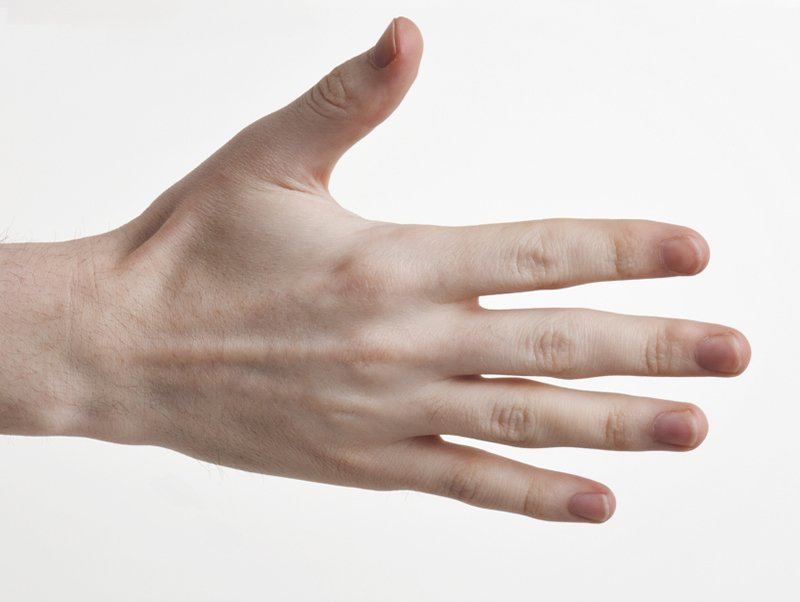
\includegraphics[width=\textwidth,height=\textheight,keepaspectratio]{../inputs/hand_pale.jpg}
  \end{minipage} & 
  \begin{minipage}{.29\textwidth}
    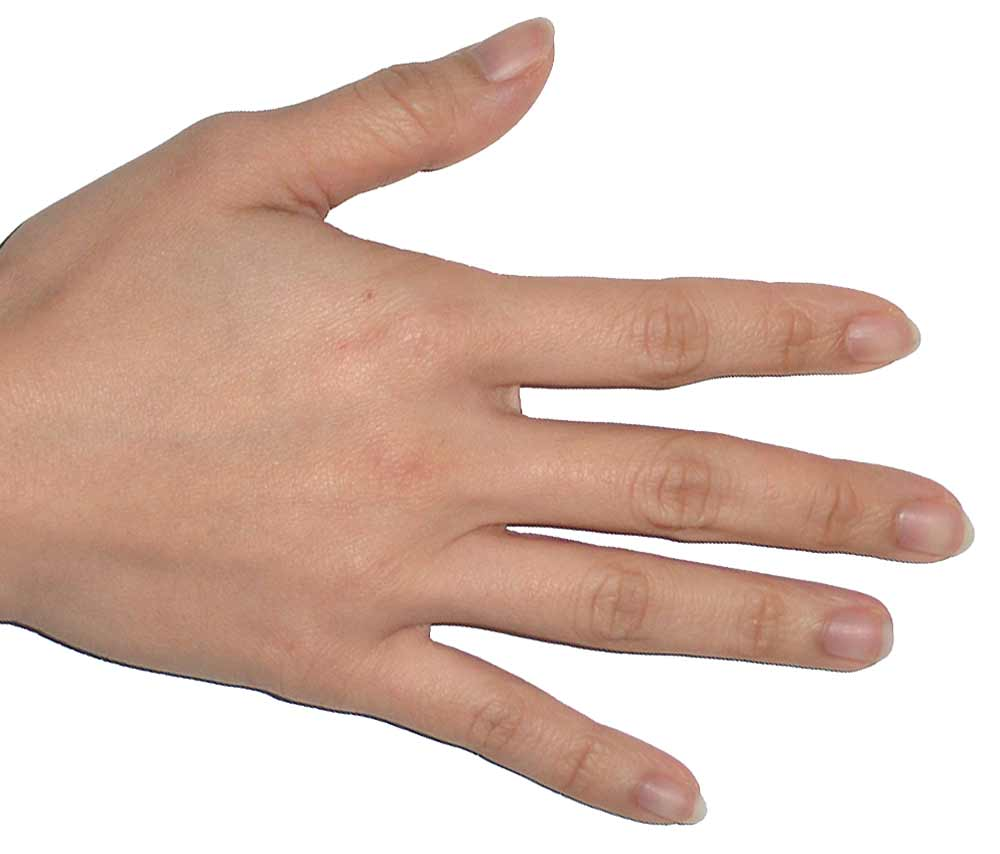
\includegraphics[width=\textwidth,height=\textheight,keepaspectratio]{../inputs/hand_light.jpg}
  \end{minipage} & 
  \begin{minipage}{.29\textwidth}
    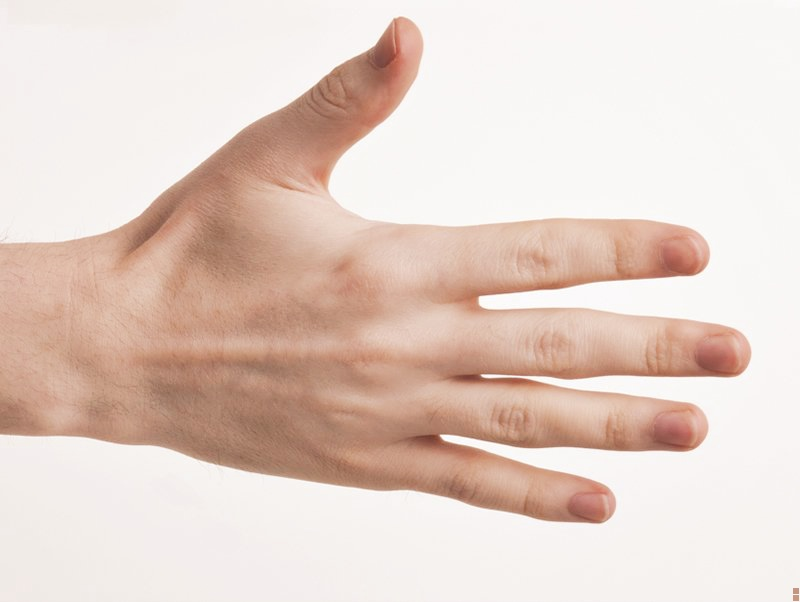
\includegraphics[width=\textwidth,height=\textheight,keepaspectratio]{../rc_test/outputs/20170522_proportional_corrected_test_alpha1p1/hand_pale_to_hand_light.jpg}
  \end{minipage} \\
\hline
 \end{longtable}

\subsubsection*{Evaluation}
As shown in Figure \ref{img:compare_dark_spot}, the dark spots and creases noted in Section \ref{sec:algo_prop_eval} are reduced.

\begin{figure}[H]
    \centering
    \begin{subfigure}[b]{0.40\textwidth}
        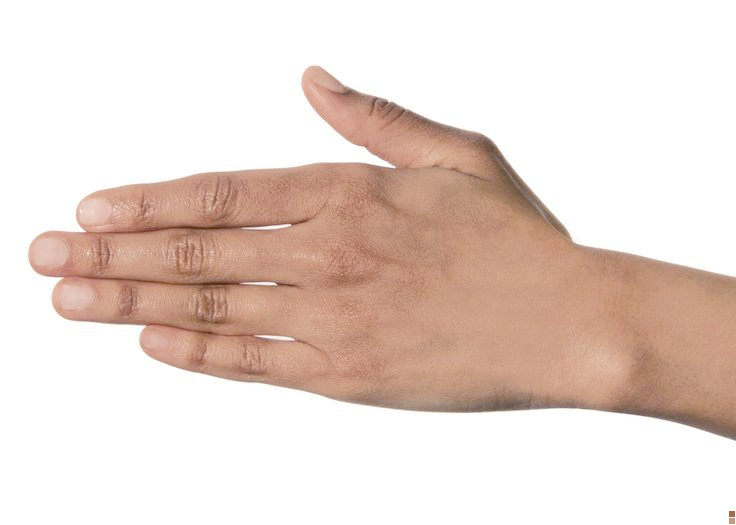
\includegraphics[width=\textwidth]{../rc_test/outputs/20170516_proportional_test/hand_brown_to_hand_light.jpg}
        \caption{Proportional adjustment algorithm (Equation \ref{eq:prop_algo})result}
    \end{subfigure}
    ~
    \begin{subfigure}[b]{0.40\textwidth}
        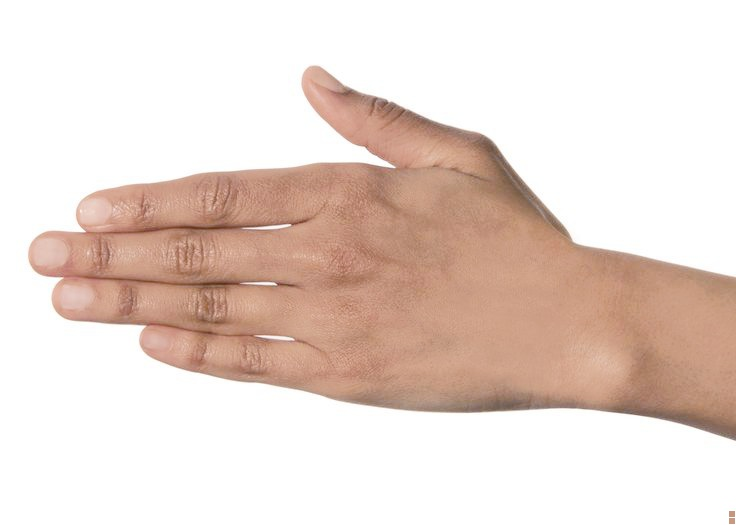
\includegraphics[width=\textwidth]{../rc_test/outputs/20170522_proportional_corrected_test_alpha1p1/hand_brown_to_hand_light.jpg}
        \caption{Proportional adjustment algorithm with correction (Equation \ref{eq:prop_corr_algo}) result}
    \end{subfigure}
    \caption{Comparison of algorithms \ref{eq:prop_algo} and \ref{eq:prop_corr_algo} results for transforming a mid-toned hand (Figure \ref{img:input_hands_1_brown}) to a light hand (Figure \ref{img:input_hands_1_light}).\label{img:compare_dark_spot}}
\end{figure}

We tried this effect for a range of $\alpha$ and found that $\alpha = 1.1$ gives an acceptably realistic result. A larger $\alpha$ would further reduce the dark spots on the skin but may begin to strongly brighten the shadows of the image, resulting in an unrealistic effect.

Up to the current iteration the more extreme changes of luminosity, such as from Figure \ref{img:input_hands_1_dark} to Figure \ref{img:input_hands_1_pale} and vice versa are especially unrealistic. Part of the reason is that the shadows, most prominent in Figure \ref{img:input_hands_1_pale} may be causing the average colour of the entire hand to be of lower luminosity than it should be. 